\documentclass[11pt,a4paper]{article}
\usepackage[margin=2.3cm]{geometry}
\usepackage{amsmath,amssymb}
\usepackage{booktabs}
\usepackage{graphicx}
\usepackage{tikz}
\usetikzlibrary{arrows.meta,positioning}
\usepackage{hyperref}
\usepackage{xcolor}
\usepackage{microtype}
\hypersetup{colorlinks=true,linkcolor=blue!60!black,citecolor=blue!60!black,urlcolor=blue!60!black}
% Generated by make_tables.py from hrt/results.json. Do not edit.
\newcommand{\TargetLabel}{Controlled lowering, 0.6 to 1.5 s}
\newcommand{\TargetL}{0.6}
\newcommand{\TargetU}{1.5}
\newcommand{\Horizon}{2}
\newcommand{\MinReps}{3}
\newcommand{\Budget}{0.5}
\newcommand{\Seed}{7}
\newcommand{\LabelVersion}{tempo-v1}
\newcommand{\FeatureVersion}{f1}
\newcommand{\PolicyVersion}{budget-v1}
\newcommand{\ModelRun}{hrt-tempo-v1-c5c7ee36-3b66ec}
\newcommand{\DatasetSha}{c5c7ee36e16a}
\newcommand{\GitCommit}{92b02fb1ff}
\newcommand{\GeneratedAt}{2026-10-25 04:22}
\newcommand{\NPeople}{10}
\newcommand{\NRecordings}{16}
\newcommand{\NAttempts}{85}
\newcommand{\NCounted}{78}
\newcommand{\NOrigins}{78}
\newcommand{\NObserved}{22}
\newcommand{\NPositive}{8}
\newcommand{\NIneligibleBaseline}{30}
\newcommand{\NIneligibleOutside}{17}
\newcommand{\NExcludedEnded}{6}
\newcommand{\NExcludedInvalid}{3}
\newcommand{\NDevRecordings}{16}
\newcommand{\NDevOrigins}{22}
\newcommand{\NDevPositive}{8}
\newcommand{\NTestRecordings}{0}
\newcommand{\NTestOrigins}{0}
\newcommand{\NTestPositive}{0}
\newcommand{\Status}{dev-cv}
\newcommand{\DevGroups}{8}
\newcommand{\Prevalence}{36\%}
\newcommand{\LambdaFull}{10}
\newcommand{\LambdaTempo}{10}
\newcommand{\LambdaPosition}{10}
\newcommand{\BrierConst}{0.479}
\newcommand{\BrierPos}{0.701}
\newcommand{\BrierTempo}{0.536}
\newcommand{\BrierFull}{0.537}
\newcommand{\LogLossConst}{1.193}
\newcommand{\LogLossPos}{6.962}
\newcommand{\LogLossTempo}{1.359}
\newcommand{\LogLossFull}{1.360}
\newcommand{\APConst}{0.236}
\newcommand{\APFull}{0.238}
\newcommand{\TauFull}{0.95}
\newcommand{\RecallFull}{0\%}
\newcommand{\FAFull}{0.00}
\newcommand{\RecallHeur}{17\%}
\newcommand{\FAHeur}{0.00}
\newcommand{\AlertsHeur}{1}
\newcommand{\EventsDev}{6}
\newcommand{\LeadHeur}{18.0}
\newcommand{\CIBrierFullConst}{+0.048 [+0.007, +0.085]}
\newcommand{\CIBrierFullPos}{-0.128 [-0.258, +0.002]}
\newcommand{\CIRecallFullHeur}{-0.161 [-0.500, +0.000]}
\newcommand{\CIFAFullHeur}{+0.000 [+0.000, +0.000]}
\newcommand{\BootN}{1000}
\newcommand{\CalibrationStatus}{preliminary: too few events per class to assess or fit calibration}
\newcommand{\MAERidge}{0.87}
\newcommand{\MAELast}{0.25}
\newcommand{\MAEMedian}{0.26}
\newcommand{\BaselineRows}{A constant (training prevalence) & 22 & 0.479 & 1.193 & 0.236 & 0\% & 0.00 \\
B set position & 22 & 0.701 & 6.962 & 0.236 & none & -- \\
tempo features & 22 & 0.536 & 1.359 & 0.238 & 0\% & 0.00 \\
D tempo + pose (deployed) & 22 & 0.537 & 1.360 & 0.238 & 0\% & 0.00 \\
C slow-ascent rule & 22 & -- & -- & -- & 17\% & 0.00 \\
always silent & 22 & -- & -- & -- & 0\% & 0.00 \\}
\newcommand{\PerGroupRows}{kb\_racked\_squat\_01 & 1 & 0 & 0.147 & 0.153 \\
kb\_side & 2 & 2 & 0.490 & 0.465 \\
overhead\_kb\_squat\_single\_arm\_01 & 12 & 0 & 0.659 & 0.562 \\
screen\_cam/team-1 & 3 & 2 & 0.338 & 0.333 \\
screen\_cam/team-2 & 1 & 1 & 0.445 & 0.425 \\
screen\_cam/team-3 & 1 & 1 & 0.435 & 0.425 \\
squat\_frontal\_raise\_01 & 1 & 1 & 0.438 & 0.425 \\
squat\_jump\_army\_front\_01 & 1 & 1 & 0.444 & 0.425 \\}
\newcommand{\ReliabilityRows}{0.0--0.2 & 0 & not evaluated & not evaluated \\
0.2--0.4 & 10 & 0.33 & 0.80 \\
0.4--0.6 & 0 & not evaluated & not evaluated \\
0.6--0.8 & 1 & 0.80 & 0.00 \\
0.8--1.0 & 11 & 0.81 & 0.00 \\}
\newcommand{\ProvenanceRows}{barbell\_squat\_powerlifting\_comp\_01 & dev & cc-1 & imported & 2 \\
demo\_front & dev & cc-3 & imported & 2 \\
goblet\_squat\_kb\_01 & dev & cc-4 & imported & 2 \\
half\_squat\_home\_cdc\_01 & dev & cc-5 & imported & 6 \\
kb\_clean\_squat\_thruster\_01 & dev & cc-4 & imported & 3 \\
kb\_complex\_ia\_01 & dev & cc-6 & imported & 2 \\
kb\_racked\_squat\_01 & dev & cc-4 & imported & 5 \\
kb\_side & dev & cc-4 & imported & 6 \\
overhead\_kb\_squat\_01 & dev & cc-4 & imported & 1 \\
overhead\_kb\_squat\_single\_arm\_01 & dev & cc-4 & imported & 16 \\
overhead\_kb\_waiters\_squat\_01 & dev & cc-4 & imported & 1 \\
screen\_cam/team-1 & dev & team-1 & live-recorded & 7 \\
screen\_cam/team-2 & dev & team-2 & live-recorded & 8 \\
screen\_cam/team-3 & dev & team-3 & live-recorded & 6 \\
squat\_frontal\_raise\_01 & dev & cc-8 & imported & 6 \\
squat\_jump\_army\_front\_01 & dev & cc-9 & imported & 5 \\}
\newcommand{\LabelDefinition}{v\_t = 1 when the lowering duration of counted rep t is outside [0.6, 1.5] s; Y\_t = 1 when v = 1 for rep t+1 or t+2; origins need 3 counted reps and v\_t = 0; horizons with an uncounted attempt or fewer than 2 further reps are excluded.}


\title{Spottr: Short-Horizon Exercise Forecasting and Coaching Decisions Under an Interruption Budget}
\author{Nakki (NakkiV7) with the Spottr team \\ OxHack '26, 25 October 2026}
\date{}

\begin{document}
\maketitle

\begin{abstract}
A camera-based squat coach measures the lowering phase of every repetition. We ask whether those measurements, available as soon as a repetition ends, forecast that the lowering tempo of one of the next two repetitions will leave a programme's target range, and whether that forecast is worth interrupting the person with a cue. We define the forecast origin, the two-rep horizon, the exclusion rules for incomplete horizons, and a compact feature set that uses only repetitions already completed. An $L_2$-regularised logistic regression is compared with a constant baseline, a set-position baseline and the coach's existing reactive slow-ascent rule, under grouped cross-validation over recordings with a paired cluster bootstrap. On the development material available at submission (\NRecordings{} recordings of \NPeople{} people, \NCounted{} counted repetitions, \NDevOrigins{} eligible origins of which \NDevPositive{} are positive) the logistic model is worse than the constant baseline (Brier \BrierFull{} against \BrierConst{}; bootstrap difference \CIBrierFullConst), no threshold satisfies the false-alert budget of \Budget{} per set, and the deployed policy therefore stays silent, while the existing rule recalls \RecallHeur{} of events with \FAHeur{} false alerts per set. The infrastructure that turns this into a decision runs end to end: forecasts are emitted in shadow mode at every eligible origin, persisted in TimescaleDB before their outcome exists, resolved when the horizon closes, shown in a post-set review and an evidence panel, and replayed from held-out recordings using only the prefix played so far. A locked held-out evaluation awaits recordings that had not been made at submission. We claim no prediction of fatigue, injury or muscular failure; the target is a tracker-derived tempo criterion.
\end{abstract}

\section{Motivation}

A coach who speaks after a repetition has already gone wrong is reacting; a coach who speaks before it has a chance to change it. The difference is a forecast, and the cost of a forecast is interruption: every unnecessary cue teaches the person to ignore the next one. The decision we study is therefore not ``is the next rep bad?'' but ``is the evidence that it may be bad strong enough to spend one interruption on?'' That is a sequential decision problem under a budget, made once per repetition, with information that grows by one observation each time. The hackathon's theme of time runs through every part of it: the model learns from the repetitions before, forecasts the two after, decides whether to speak now, and is scored later by how long before the event its warning came.

We keep the formulation deliberately small. One exercise (the squat), one measured quantity (the lowering duration), one programme target, one horizon of two repetitions, one linear model, and three baselines that any claimed improvement must beat under the same budget. A small, reproducible, negative result is preferable to an elaborate one nobody can check.

\section{System and data}

\begin{figure}[t]
\centering
\resizebox{\linewidth}{!}{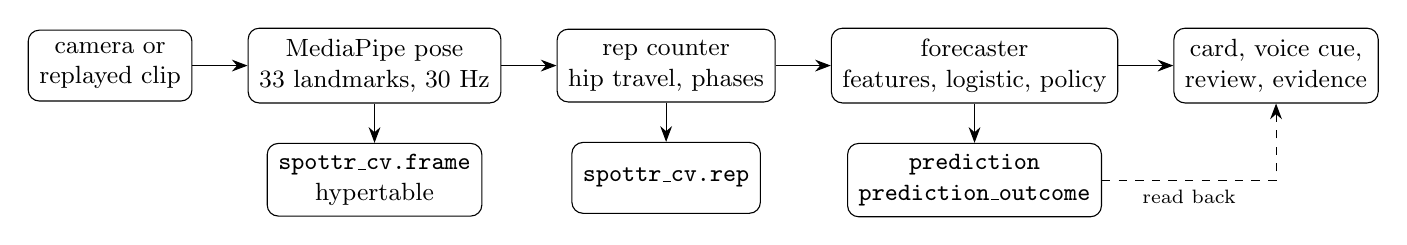
\begin{tikzpicture}[node distance=5mm and 7mm, box/.style={draw, rounded corners, align=center, font=\small, inner sep=4pt, minimum height=9mm}, >={Stealth[length=2mm]}]
\node[box] (cam) {camera or\\replayed clip};
\node[box, right=of cam] (pose) {MediaPipe pose\\33 landmarks, 30 Hz};
\node[box, right=of pose] (rep) {rep counter\\hip travel, phases};
\node[box, right=of rep] (fc) {forecaster\\features, logistic, policy};
\node[box, below=of pose] (frames) {\texttt{spottr\_cv.frame}\\hypertable};
\node[box, below=of rep] (reps) {\texttt{spottr\_cv.rep}};
\node[box, below=of fc] (pred) {\texttt{prediction}\\\texttt{prediction\_outcome}};
\node[box, right=of fc] (ui) {card, voice cue,\\review, evidence};
\draw[->] (cam) -- (pose); \draw[->] (pose) -- (rep); \draw[->] (rep) -- (fc); \draw[->] (fc) -- (ui);
\draw[->] (pose) -- (frames); \draw[->] (rep) -- (reps); \draw[->] (fc) -- (pred);
\draw[->, dashed] (pred) -- node[below, font=\scriptsize] {read back} (ui |- pred) -- (ui);
\end{tikzpicture}}
\caption{Data flow. Everything left of the database runs in the browser; the database is TimescaleDB on Tiger Data. The forecaster writes its forecast before the next repetition can be observed, and the review and evidence views read the stored rows rather than the page's memory.}
\label{fig:system}
\end{figure}

\paragraph{Measurements.} Pose is estimated per frame with MediaPipe Pose Landmarker (full model) \cite{bazarevsky2020,mediapipedocs}. The squat counter tracks hip height above the ankle in units of standing leg length (``hip travel''). A repetition starts when travel exceeds 0.15, reaches its bottom when travel has come back 0.04 below its maximum, and ends when travel drops below 0.08. The lowering duration $d_t$ of repetition $t$ is the time from start to bottom; the rising duration is the time from bottom to end. Both are reported to 0.1~s. Attempts that do not reach 0.22 of leg length, or last under 0.5~s or over 15~s, are recorded as attempts that did not count. Depth (hip below knee, in thigh lengths), lean and knee tracking are graded per repetition but are only judged when the relevant joints are inside the frame; otherwise they are missing, not zero.

\paragraph{Storage.} Every analysed frame, every attempt and every set are rows in a \texttt{spottr\_cv} schema on TimescaleDB \cite{timescaledocs}: a frame hypertable at about 30 rows per second, a repetition hypertable with both phase durations, and a workout table. Real-time continuous aggregates roll frames up per second and repetitions up per minute. Forecasts and outcomes are two further tables: a forecast row is written once, with the instant after which no information was used, and is never updated; an outcome row is added when the horizon closes and points at its forecast. A model-run table records the deployed artifact, its data fingerprint and its evaluation summary.

\paragraph{Recordings.} At submission the dataset consists of \NRecordings{} recordings: 16 Creative Commons clips of squats from Wikimedia Commons and YouTube (different people, loads, camera angles and distances), and one webcam session of three team members in turn, split into three recordings by the gaps between them. All were used to tune the repetition counter and are therefore development material. Each recording is one sampling unit (one person, one set); nothing in the evaluation treats frames, or overlapping windows within a set, as independent. Provenance is listed in Table~\ref{tab:prov}.

\section{Problem formulation}

Let $d_t$ be the lowering duration of counted repetition $t$ in a set and $[L,U]$ the programme's acceptable range, here \TargetLabel{} ($L=\TargetL$, $U=\TargetU$~s). The range is a prescription chosen before the experiment; it is not a definition of safe or correct technique. Define the violation indicator
\begin{equation}
v_t = \mathbb{1}\{d_t < L \ \text{or}\ d_t > U\}.
\end{equation}
After repetition $t$ the forecaster emits
\begin{equation}
p_t = P\big(Y_t = 1 \mid \mathcal{I}_t\big), \qquad Y_t = \max(v_{t+1}, v_{t+2}),
\end{equation}
where $\mathcal{I}_t$ is the information available at the end of repetition $t$. An origin $t$ is \emph{eligible} when at least \MinReps{} counted repetitions have been completed, $v_t = 0$ (the forecast is of onset, not of continuation of a deviation already under way), and the variation and target have not changed within the set. $Y_t$ is \emph{observed} only when the next two physical attempts are both counted repetitions. If the set ends first, or an attempt in the horizon does not count, the origin is excluded with that reason and never labelled negative. We do not redefine the horizon by skipping attempts that did not count. Stopping and tracking loss may be informative; their counts are reported, and the complete-horizon rule is the primary experiment's convention.

\section{Features and model}

The feature vector at an eligible origin uses only counted repetitions $1,\dots,t$ (feature version \FeatureVersion, window 3): the latest lowering duration; the median of the last three; the latest minus the median of the previous repetitions (trend); the range of the last three; the normalised distance to the nearer edge of the target, $\min(d_t - L, U - d_t)/(U-L)$; the latest rising duration and its trend; the repetition number; the time since the first repetition began; the change in depth against the median of the previous repetitions; and an indicator for depth not being judged. No cross-session personal baseline is used yet, so the first three repetitions of every set are a cold start. The same function computes features for the offline experiment and in the page; a unit test asserts they agree, and another asserts that changing repetitions after the origin cannot change its features.

The primary model is logistic regression with an $L_2$ penalty on standardised features,
\begin{equation}
p_i = \sigma(\beta_0 + \mathbf{x}_i^{\top}\boldsymbol\beta), \qquad
\min_{\beta_0,\boldsymbol\beta}\; -\frac{1}{n}\sum_{i=1}^{n}\big[y_i \log p_i + (1-y_i)\log(1-p_i)\big] + \lambda\lVert\boldsymbol\beta\rVert_2^2,
\end{equation}
with the intercept unpenalised so that the fitted base rate is not shrunk \cite{hastie2009}. Standardisation statistics are computed on the training recordings only; a missing feature value is imputed as the training mean (zero after standardisation) and, for depth, is accompanied by the missing indicator. The penalty $\lambda \in \{0.01, 0.1, 1, 10\}$ is chosen by nested leave-one-recording-out log loss inside each training fold. Coefficients are associational: they describe which observations move the forecast, not what causes a tempo miss. No class weights or oversampling are used, so the fitted probabilities refer to the actual event prevalence.

\section{Decision policy}

The policy has three actions: stay silent, give one permitted cue, or abstain because the origin is ineligible or tracking is unreliable. A cue is given when $p_t \ge \tau$ and no cue has been given in the previous $\Horizon{}$ repetitions. The threshold is chosen on development predictions as
\begin{equation}
\tau^{*} = \arg\max_{\tau}\; \mathrm{Recall}(\tau) \quad \text{subject to} \quad \mathrm{FalseAlertsPerMonitoredSet}(\tau) \le B, \qquad B = \Budget,
\end{equation}
with ties resolved towards the higher threshold. $B$ is a product choice (one unnecessary interruption every two sets), not a medical constant. An \emph{event} is an onset: a violating repetition preceded by a compliant one. A warning at origin $t$ matches an onset at $t+1$ or $t+2$; each onset is matched at most once, so repeated warnings are not repeated successes. A warning whose observed horizon contains no onset is a false alert; a warning whose horizon is excluded is unresolved and counted in neither. Lead time is the time from the end of the origin repetition to the end of the onset repetition. The existing reactive rule (ascent longer than 2.2~s, or 1.6 times the median of earlier ascents) is evaluated as the same kind of alerting policy at the same origins. Always-silent is included: zero false alerts, zero recall.

\section{Experimental design}

Recordings are the groups. The development evaluation is leave-one-recording-out: every origin's out-of-fold prediction comes from a model that never saw its recording, with $\lambda$ chosen inside the training fold. The baselines are (A) a Laplace-smoothed constant equal to the training prevalence, (B) a logistic model on repetition number and elapsed time only, (C) the existing slow-ascent rule, and (D) the logistic model above. Ablations use the same origins with set-position, tempo, and tempo plus pose features. Probabilistic forecasts are scored with the Brier score \cite{brier1950} and log loss, both strictly proper \cite{gneiting2007}, and average precision; policies with event recall at the budget, false alerts per monitored set, precision and lead time. Calibration is inspected with a reliability diagram with bin counts; Platt scaling \cite{platt1999} is applied only when out-of-fold predictions contain at least ten events of each class, which they do not here, so probabilities are labelled preliminary wherever they are shown. Uncertainty for differences between models comes from a paired cluster bootstrap \cite{efron1993}: recordings are resampled with replacement (\BootN{} resamples, seed \Seed), the same resampled recordings are scored under both models, and 2.5 and 97.5 percentiles of the difference are reported. Because the out-of-fold predictions are held fixed, these intervals reflect sampling of recordings, not model-selection uncertainty. The prespecified primary comparisons are D against A on Brier, and D against C on recall under the budget. A held-out test split is defined in the manifest but empty at submission; when the team's recordings are added, the frozen configuration is evaluated on them once, and any later change to labels, features, $\lambda$, $\tau$ or the budget invalidates that status.

\section{Results}

\begin{table}[t]
\centering\small
\caption{Development results, out of fold over \DevGroups{} recordings and \NDevOrigins{} eligible origins (prevalence \Prevalence). Recall at budget is event recall at the highest threshold whose false alerts per set stay within \Budget. Dashes: not a probabilistic model.}
\label{tab:baselines}
\begin{tabular}{lrrrrrr}
\toprule
model & $n$ & Brier & log loss & AP & recall at budget & false alerts/set \\
\midrule
\BaselineRows
\bottomrule
\end{tabular}
\end{table}

\begin{figure}[t]
\centering
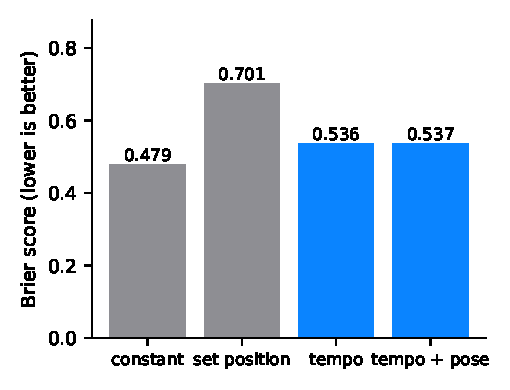
\includegraphics[width=.32\linewidth]{fig_brier.pdf}\hfill
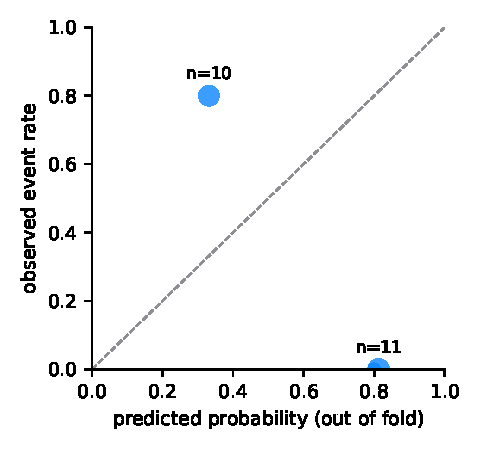
\includegraphics[width=.32\linewidth]{fig_reliability.pdf}\hfill
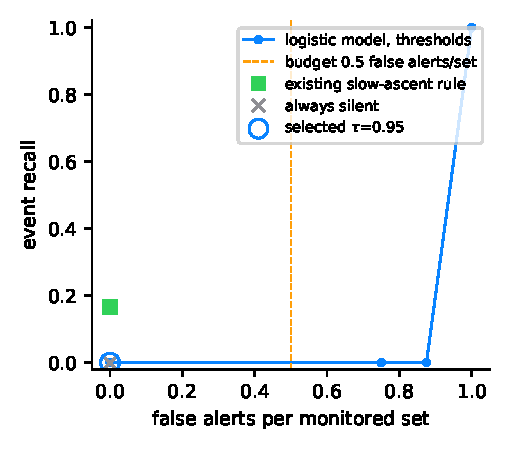
\includegraphics[width=.34\linewidth]{fig_frontier.pdf}
\caption{Left: Brier score by feature set (lower is better). Middle: reliability diagram of the deployed model's out-of-fold probabilities with bin counts; \CalibrationStatus. Right: event recall against false alerts per set over thresholds, the budget line, the existing rule and silence.}
\label{fig:results}
\end{figure}

Of \NOrigins{} counted-repetition origins, \NIneligibleBaseline{} fall in the three-repetition baseline, \NIneligibleOutside{} have a current repetition already outside the target, \NExcludedEnded{} lose their horizon to the end of the set and \NExcludedInvalid{} to an attempt that did not count, leaving \NObserved{} observed origins with \NPositive{} positive outcomes. Table~\ref{tab:baselines} and Figure~\ref{fig:results} give the development results. The deployed model's Brier score is \BrierFull{} against \BrierConst{} for the constant baseline; the bootstrap interval of the difference, \CIBrierFullConst, excludes zero on the wrong side: the model is worse. The set-position baseline is worse still (\BrierPos, log loss \LogLossPos), with extreme out-of-fold probabilities from fitting two features on a handful of recordings. Average precision is \APFull{} for the model and \APConst{} for the constant, i.e.\ no ranking signal. Under the budget of \Budget{} false alerts per set, the only admissible threshold for the model is \TauFull, at which it alerts on nothing (recall \RecallFull); the existing slow-ascent rule alerts \AlertsHeur{} time(s) in \EventsDev{} events with recall \RecallHeur{} and \FAHeur{} false alerts per set, a median lead of \LeadHeur{}~s. The recall difference, model minus rule, is \CIRecallFullHeur. Per-recording Brier scores (Table~\ref{tab:pergroup}) show the pattern: one long recording of 16 repetitions supplies most origins and most negatives, and leaving it out removes most of the training set.

As a separately reported fallback, a ridge regression of the next lowering duration on the tempo features has mean absolute error \MAERidge{}~s out of fold, against \MAELast{}~s for repeating the last duration and \MAEMedian{}~s for the rolling median: persistence wins. Prediction latency in the page is below one millisecond after the repetition event (median 0.5~ms in the stored replay), so the horizon is never consumed by computation.

\begin{table}[t]
\centering\small
\caption{Per-recording out-of-fold Brier scores, deployed model against the constant baseline.}
\label{tab:pergroup}
\begin{tabular}{lrrrr}
\toprule
recording & origins & positives & Brier (model) & Brier (constant) \\
\midrule
\PerGroupRows
\bottomrule
\end{tabular}
\end{table}

\paragraph{Held-out test.} \ifdefined\TestGroups Evaluated once on \TestGroups{} held-out recordings (\NTestOrigins{} origins, prevalence \TestPrevalence): Brier \TestBrierFull{} (model) against \TestBrierConst{} (constant), log loss \TestLogLossFull; at the frozen threshold the model's recall is \TestRecallFull{} with \TestFAFull{} false alerts per set, the rule's \TestRecallHeur{} with \TestFAHeur. \else Not evaluated: no held-out recordings existed at submission. The split is reserved in the manifest and the configuration above is frozen; the evaluation runs once when the recordings arrive. \fi

\paragraph{Failure cases.} The data do not contain enough naturally occurring onsets to distinguish a slow drift from an isolated fast descent; most positives in the development set are single repetitions in otherwise compliant sets of unrelated people, which no feature of the previous three repetitions anticipates. Camera cuts, pick-ups and walk-ins are filtered by the counter before the forecaster sees them, but every such filter reduces the horizon coverage reported above.

\section{User-facing system}

\begin{figure}[t]
\centering
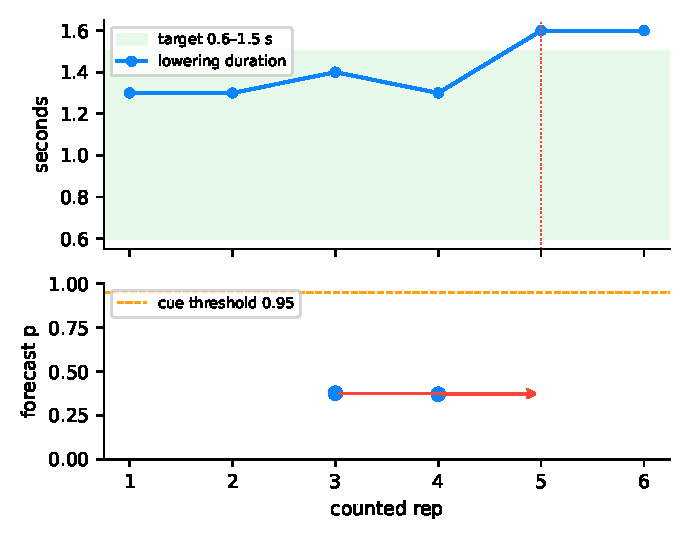
\includegraphics[width=.72\linewidth]{fig_timeline.pdf}
\caption{A stored shadow-mode replay of a held-out Creative Commons clip (6 repetitions). Top: lowering duration per repetition against the target band; dotted lines mark onsets. Bottom: the forecast probability at each eligible origin and, for observed positives, an arrow to the onset it preceded (lead times 16.4~s and 8.5~s). The dashed line is the frozen cue threshold, which no forecast crossed. All values are read from the database, not from the page.}
\label{fig:timeline}
\end{figure}

The forecaster runs inside the existing squat page. A compact card below the repetition counter shows one of six states, updated only at repetition boundaries: learning your pace ($n$ of 3), tracking your next reps, a cue, the last rep was outside the range, a framing problem (hips and knees not tracked), or prediction unavailable. The card never uses danger styling, and its ``Why this?'' expansion names the forecast criterion, the horizon, the last three lowering durations against the target, the trend, the model identifier, the latency, and the probability labelled as preliminary and uncalibrated. In \emph{shadow mode} the forecaster records every eligible forecast and says nothing; in \emph{coaching mode} a forecast at or above the threshold speaks one cue through the existing voice queue (priority, no overlap, expiry, stop interrupts), at most once per horizon, and outcomes after a cue are flagged as observed after coaching. The set summary gains ``What we anticipated'': for each stored forecast, the repetition after which it was made, whether it would have cued, what was observed, the lead time, horizons left incomplete, and onsets that had no eligible warning. An \emph{Evidence} dialog renders the saved evaluation artifact (Table~\ref{tab:baselines}, the bootstrap intervals, reliability, the decision frontier, ablations, the dataset card and reproducibility identifiers) and the stored timeline of the last set (Figure~\ref{fig:timeline}). A replay mode plays a held-out clip once and pauses at every forecast before the following repetitions are shown; because the counter has not seen the rest of the clip, every forecast in the replay uses only the prefix that has played.

\section{Discussion and limitations}

The honest summary is that the infrastructure is finished and the model is not supported by the data. With \NDevOrigins{} origins from \DevGroups{} recordings of different people, loads and camera placements, a linear model of recent tempo cannot beat a constant, and the budgeted policy correctly refuses to speak. Three limitations dominate. First, labels are produced by the repetition counter, not by independent annotation: a ``tempo miss'' is whatever the tracker measures at 0.1~s resolution, and the forecast is of that measurement. Second, the development clips were used to tune the counter, so even the development numbers are optimistic about tracking quality. Third, the recordings are not sets of one person getting tired; they are short sets of many people, which is the wrong population for a fatigue-driven drift and the right population only for the cold-start behaviour. Overlapping horizons within a set are correlated, which is why uncertainty is computed over recordings; informative stopping (a set ending because the person felt the next repetition would miss) is excluded rather than modelled. Nothing here estimates a causal effect of the cue, which would require intervention data, and nothing here predicts physiological failure.

What would change the picture is simple to state: sets recorded to ordinary volitional stopping by a handful of people, split by person into development and locked test, which is the plan for the recordings being made after submission. A discrete-time survival formulation of repetitions until the first miss, with the risk set and censoring treated properly, is future work that the same stored records would support.

\section{Reproducibility}

\begin{sloppypar}
Commit \GitCommit; dataset fingerprint \DatasetSha; model \ModelRun; label \LabelVersion, features \FeatureVersion, policy \PolicyVersion; evaluated \GeneratedAt{} UTC with seed \Seed. From \texttt{prototype/squat}: \texttt{node hrt/build\_dataset.mjs <landmark-dir>} writes the repetition dataset from landmark dumps whose SHA-256s are committed; \texttt{node hrt/train.mjs} writes \texttt{hrt/model.json} and \texttt{hrt/results.json}; \texttt{npm test} runs 39 offline checks. This document's numbers are macros generated from \texttt{results.json} by \texttt{make\_tables.py}, and its figures by \texttt{make\_figures.py}; Node 26, Python 3.15 with matplotlib, Tectonic 0.17.
\end{sloppypar}

\appendix
\section{Dataset provenance and label}

\LabelDefinition

\begin{table}[h]
\centering\small
\caption{Recordings. Person identifiers are anonymous; ``imported'' recordings are Creative Commons clips, ``live-recorded'' the team session.}
\label{tab:prov}
\begin{tabular}{lllll}
\toprule
recording & split & person & provenance & counted reps \\
\midrule
\ProvenanceRows
\bottomrule
\end{tabular}
\end{table}

\begin{table}[h]
\centering\small
\caption{Reliability bins of the deployed model's out-of-fold probabilities.}
\begin{tabular}{lrrr}
\toprule
bin & $n$ & mean predicted & observed \\
\midrule
\ReliabilityRows
\bottomrule
\end{tabular}
\end{table}

\bibliographystyle{plain}
\bibliography{references}
\end{document}
